\documentclass[sigconf]{acmart}

\usepackage{booktabs} % For formal tables
\usepackage[utf8]{inputenc}
\usepackage[british]{babel}
\usepackage{graphicx,url}
\usepackage[linesnumbered,ruled,vlined]{algorithm2e}

\usepackage{amsmath}
\usepackage{breqn}


% Copyright
%\setcopyright{none}
%\setcopyright{acmcopyright}
%\setcopyright{acmlicensed}
\setcopyright{rightsretained}
%\setcopyright{usgov}
%\setcopyright{usgovmixed}
%\setcopyright{cagov}
%\setcopyright{cagovmixed}


% DOI
\acmDOI{10.475/123_4}

% ISBN
\acmISBN{123-4567-24-567/08/06}

%Conference
\acmConference[NanoCOM'2018]{ACM NanoCOM conference}{September 2018}{Reykjavik, Iceland}
\acmYear{2018}
\copyrightyear{2018}


\acmArticle{4}
\acmPrice{15.00}

% These commands are optional
%\acmBooktitle{Transactions of the ACM Woodstock conference}
\editor{Jennifer B. Sartor}
\editor{Theo D'Hondt}
\editor{Wolfgang De Meuter}


\begin{document}
\title{MAC-Protocol for Traffic regulation in Ultra-Dense Nanonetwork}


\author{Lina Aliouat}
\affiliation{%
  \institution{Univ. Bourgogne Franche-Comt\'e}
  \streetaddress{1 Cours Leprince Ringuet}
  \city{Montb{\'e}liard}
  \country{France}
  \postcode{25200}
}
\email{lina.aliouat@femto-st.fr}

\author{Hakim Mabed}
\affiliation{%
  \institution{Univ. Bourgogne Franche-Comt\'e}
  \streetaddress{1 Cours Leprince Ringuet}
  \city{Montb{\'e}liard}
  \country{France}
  \postcode{25200}
}
\email{hmabed@femto-st.fr}

\author{Julien Bourgeois}
\affiliation{%
  \institution{Univ. Bourgogne Franche-Comt\'e}
  \streetaddress{1 Cours Leprince Ringuet}
  \city{Montb{\'e}liard}
  \country{France}
  \postcode{25200}
}
\email{julien.bourgeois@femto-st.fr}


% The default list of authors is too long for headers.
%\renewcommand{\shortauthors}{H. Mabed, al.}


\begin{abstract}
Les réseaux nano terahertz représentent un des axes prometteurs dans le domaine des télécommunication sans fils. Les avancées technologiques réalisées dans la miniaturisation des antennes et les communications terahertz ont ouvert la voie à de nouvelles applications réseau tels que le Body network, la matière programmable ou encore les processeurs muti-core. Certaines de ces applications nécessitent la concentration d'un nombre très élevés de noeuds minuscules dans un espace limité. Dans ce context ultra dense et en l'abscence d'unités de contrôle d'accès, nous proposons de définir une stratégie distribuée de régulation spatiale et temporelle du trafic pour se prémunir des risques de congestion, d'interférences et de sur-consomation d'énergie. Nous proposons dans cette article un protocole d'optimisation des liaisons radio permettant à la fois de réduire le flux de trafic unutil sur le réseau, d'aplanir dans le temps le volume de communications échangées et préserver la durée de vie des noeuds.  
\end{abstract}

%
% The code below should be generated by the tool at
% http://dl.acm.org/ccs.cfm
% Please copy and paste the code instead of the example below.
%
\begin{CCSXML}
<ccs2012>
<concept>
<concept_id>10003033.10003039.10003044</concept_id>
<concept_desc>Networks~Link-layer protocols</concept_desc>
<concept_significance>300</concept_significance>
</concept>
</ccs2012>
\end{CCSXML}

\ccsdesc[300]{Networks~Link-layer protocols}

\keywords{Terahertz Nanonetwork, Ultra Dense nanonetwork, directional antenna, MAC Layer}


\maketitle

\section{Introduction}

De nouvelles applications réseau ont vu le jour ces dernières années portées par les avancées majeures de la miniaturisation des équipements électroniques et des antennes radio. Dans ce type de systèmes réseau, un nombre très élevés d'équipements radio sont confinés dans un espace réduit. Dans ce contexte, la bande de fréquences Térahertz résente le double avantage d'allier une bande passante élevée avec une portée énergétique et spatiale faible. Dans le domaine de la matière programmable, par exemple, un nombre élevé de micro-robots sont capables de se réorganiser en différentes formes. Les algorithmes distribués de réorganisation peuvent être largement améliorés par l'utilisation de procédures de communication non restreintes au noeuds voisins. L'utilisation des communications térahertz à courte portée trouve aussi une application dans le domaine des architectures informatiques massivement multi-coeur. L'idée est alors de déployer un grand nombre de processeurs sur une même puce et remplacer les bus de communication classiques par des liaisons radio à très haut débit \cite{abadal}. 

En raison des capacités de calcul et d'énergie restreintes des nœuds du réseau, les protocoles d'accès multiple doivent répondre à des exigences de simplicité et de scalabilité. L'accès au canal doit se faire en réduisant le nombre de messages de contrôle et sans recourir à des entités de centralisation. Pour répondre à ce besoin, plusieurs techniques innovantes ont été proposées telles que : TS-OOK, ASRH-TSOOK, Smart-MAC, Wise-MAC ... Ces travaux proposent des politiques de partage du canal permettant aux nœuds de définir les paramètres de la communication : quand commencer à émettre ? sur quelle canal logique ? etc.

Cependant, en vu de la densité extrême du réseau, les protocoles d'accès multiple ne sont pas en mesure de répondre au besoin de maîtrise des flux multi-saut sur le réseau. En effet, vu la densité du réseau, la diffusion de message provoque des boucles de renvoie d'un même message saturant ainsi le système (tempêtes de diffusion). Nous proposons dans cet article une procédure complémentaire à la couche MAC que nous pourrons décrire comme un protocole de couche 2.5. L'idée est de définir la topologie logique optimale du réseau permettant à la fois de réguler le trafic sur le réseau tout en conservant sa robustesse. La régulation du trafic sur le réseau vise à :
  
\begin{itemize}
\item Maîtriser la circulation des flux dans le temps : que ce soit face à des évènements de communication interdépendants ou des flux de trafic en chaîne, le trafic sur les réseaux présente des pics temporels engendrant des phénomènes de congestion. Le principe de prise de rendez-vous et d’accès multiple par division de temps (TDMA), permet de contrôler et de planifier dans le temps les communications.
\item Maîtriser la circulation des flux dans l’espace : le réseau dense présente une multitude d’itinéraires pour l’acheminement de données depuis un noeud à un autre. Sur le plan de routage, ceci implique une plus grande complexité de choix. Les risque de congestion locale sur le réseau est donc élevé. De plus pour des actions de diffusion (broadcast), la multiplication des itinéraires possibles implique plus de redondance des retransmissions (multiple réception d’un même message par différentes sources). La directionalité des antennes permet de mieux maîtriser l'impact des signaux radio émis (interférence) tout en sélectionnant les noeuds destinataire du message. 
\item Maîtriser la consomation d'énergie : la communication par rendez-vous, permet à un nœud de planifier les moments d’éveil correspondant aux périodes propices à la réception des données et aux périodes prévues pour les émissions. L'énergie consommé par les communications est réduite car la puissance émise est canalisé dans une direction spécifique à un moment donné.
\end{itemize}

La régulation du trafic revient donc à définir une topologie logique du réseau qui à partir de la topologie physique (deux nœuds peuvent communiquer dès lors qu'ils sont à portée l'un de l'autre), désigne un sous ensemble de noeuds voisins qui peuvent communiquer dans un sens prédéterminé et à des périodes prédéterminées. De ce point de vue, la topologie logique représente un sous-graphe orienté de la topologie physique. La robustesse la topologie logique renvoie premièrement à la connexité du sous-graphe. Deuxièmement, la topologie logique doit garantir que chaque nœud puissent être joignable (destination des arcs) et pouvoir joindre (source des arcs) suffisamment de nœuds. Cette propriété permet de vérifier que la topologie logique est suffisamment stable face aux risques de pannes. 

Des protocoles de régulation de trafic pour les réseaux ad hoc ont été proposé dans la littérature \cite{oslr}. L'un des plus connu est le protocole Optimized Link State Routing (OLSR) \cite{olsr}. L'utilisation de ce protocole dans le cas d'un réseau ultra-dense s'avère compliquée. OLSR se base sur l'échange des listes de voisins à proximité de chaque noeud. Des listes qui dans le cas des réseaux denses sont lourdes à transmettre et difficilement stockées ou traitées. 


\section{Formalisation du problème de régulation du trafic dans les réseaux nano sans-fils}
Soit $R$ un réseau nano sans fils composé de $N$ noeuds. Chaque noeud du réseau est doté d'une antenne directionnelle reconfigurable permettant d'orienter l'antenne d'une façon dynamique et selective pour couvrir une zone en particulier. Soit $T_{rec}$ le temps nécessaire pour changer de configuration à une antenne. Soit $G(X,A)$, le graphe connexe décrivant la topologie physique du réseau avec $X$ l'ensemble des noeuds ($|X|=N$) et $A$ les liens de portée entre les noeuds. $(x,y) \in A$ signifie qu'il exite une configuration des antennes des noeuds $x$ et $y$ permettant aux deux nœuds de communiquer directement. 

Le problème de régulation du trafic consiste à calculer un sous graphe orienté $G'(X,E)$ avec $(x,y)\in E \rightarrow (x,y)\in A$ tel que les conditions suivantes soit satisfaites :
\begin{itemize}
\item $G'$ est connexe : quel que soit deux noeuds du graphe, il existe un moyen d'acheminer les données d'un noeud vers l'autre.
\begin{dmath}
 $\forall x,y \in X, \exists \text{ un chemin de }x \text{ vers }y$
\end{dmath}
\item $G'$ est robuste : quel que soit le nœud il existe suffisamment de moyens pour qu'il reçoivent les données venant des autres noeuds et suffisamment de moyens pour qu'il diffuse ses propres données.
\begin{dmath} 
$\forall x \in X, \exists y_1 ... y_p, (y_i,x) \in E and$
$\forall x \in X, \exists y_1 ... y_s, (x,y_i) \in E$
\end{dmath}
La valeur $p$ et $s$ désignent le niveau de robustesse souhaité représenté par le nombre de prédécesseurs et de successeurs de chaque noeud. Le choix d'une valeur grande de $p$ et $s$ permet un plus haut niveau de robustesse et dérive du niveau de fiabilité des noeuds. Quand les noeuds sont sujettes à des risques élevés de pannes ou si les capacités énérgétiques de noeuds font qu'il sont régulièrement en attente de recharge, alors une valeur de $p$ et $s$ élevée est préférable.
\end{itemize}

\begin{figure}[h]
\centering
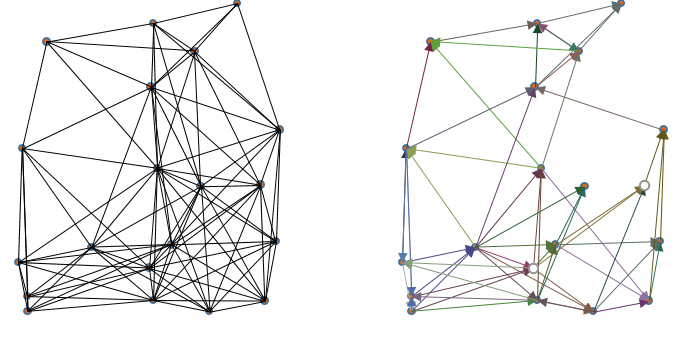
\includegraphics[width=\columnwidth]{logicaltopology.png}
\caption{Traffic regulation problem : from physical to logical topology}
\label{logicaltopology}
\end{figure}


A chaque arc $(x,y)$ du graphe $G'$ est associé deux indices (ou couleur) désignant la période de temps pendant laquelle $x$ et $y$ peuvent communiquer suivant un paramétrage particulier de leurs antennes. Chaque noeud change les paramètres de son antenne d'une façon cyclique et à intervalle de temps régulier $T_s$ suivant les différents paramètres associés aux indices. Pendant la période $S_1$, le noeud utilise le paramètrage $P_1$ puis pendant la durée $S_2$, il utilise le paramètrage $P_2$ et ainsi de suite. A la fin de la période $S_{NS}$ ($NS$ est le nombre de périodes dans un cycle), le noeud reprend de nouveau le paramètrage $P_1$ pendant une nouvelle période $S_1$ et le cycle redémarre (figure \ref{trafficregulation}). La durée d'un cycle complet $T_{c}$ est identique pour tout les noeuds (equation \ref{eqtc}). Certaines périodes $S_i$ peuvent correspondre à des périodes de veil pendant lesquelles les péréphériques de communication sont désactivés. Par ailleurs, le cycle d'un noeud peut comporter plusieurs périodes avec le même paramètrage($i\neq j,  Pi=Pj$)
\begin{dmath}
T_c=NS \ times T_s
\label{eqtc}
\end{dmath}

Pendant une période $S_i$, un noeud $x$ est soit en période de réception ou d'émission mais pas les deux à la fois. Si la période $S_i$ de $x$ est une période de réception, alors il existe un seul noeud $y\in X$ tel que $(y,x)\in E$, i.e. un seul noeud écouté à la fois. Si par contre la période $S_i$ est une période d'émission de $x$, alors il existe au moins un noeud $y$ tel que $(x,y)\in E$.

Etant donnée la nature asynchrone du réseau, les périodes $S_i$ sont propores à chaque noeuds. La figure \ref{trafficregulation} montre un exemple de régulation de trafic impliquant 5 noeuds. Le noeud (A) possède deux périodes actives S_1 en émission et S_2 en réception. La période $S1=[0.3-0.4]$ couvre 1/10 de $T_{c}$ entre les instants $0.3\times T_{c}$ et $0.4\times T_{c}$. Pendant cette péiode, le noeud (A) couvre le noeud (C) qui est à l'écoute pendant sa période $S_3=[0-0.1]$ ainsi que le noeud (E) qui écoute pendant sa période $S_1=[0.7-0.8]$. 

\begin{figure}[h]
\centering
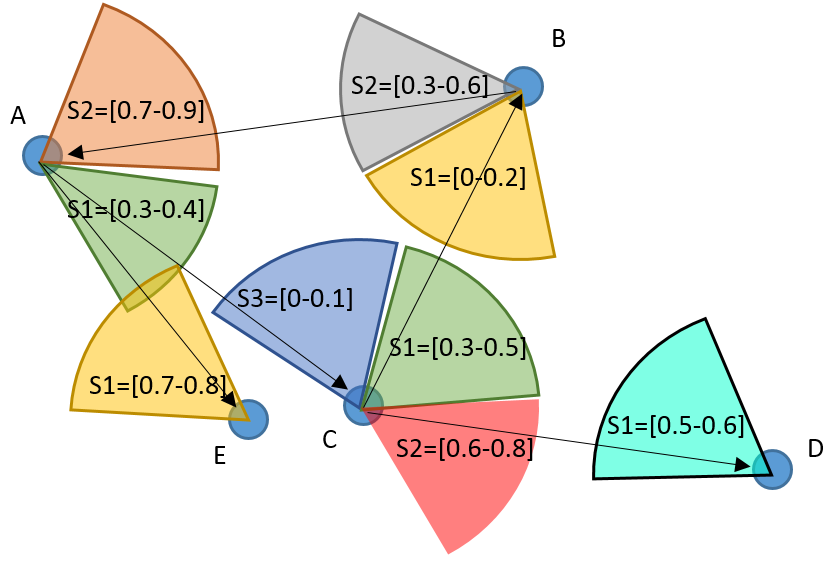
\includegraphics[width=\columnwidth]{trafficregulation.png}
\caption{Exemple of TDMA synchronization}
\label{trafficregulation}
\end{figure}


Quand deux arcs $(x,y1)$ et $(x,y2)$ avec la même extrémité sortante ont le même indice sur $x$, les deux noeuds entrants $y1$ et $y2$ peuvent alors être servis par un même flux multicast. Par ailleur, les arcs $(x1,y)$ et $(x2,y)$ avec la même extrémité entrante ne peuvent pas avoir le même indice de période sur le noeud $y$ pour éviter les interférences. Pour tout arc $(x,y)$, la période d'écoute associée sur $y$ doit  nécessairement être plus courte ou égale à la durée d'émission associée sur $x$ dans le but de maximiser les périodes de veil ou de rendre disponible $y$ pour une autre liaison.

Autre le respect des contraintes de régulation du trafic en particulier la connexité et la robustesse du sous-graphe G', l'algorithme de régulation de trafic doit veiller à maximiser les durées d'écoute et d'émission utiles, $T_i$, ($T_i \subset S_i$) ainsi que les périodes de veil des noeuds. Une période d'émission d'un noeud $x$ est dite utile quand sur toute sa durée, il existe toujours au moins un noeud $y, (x,y)\in E$ à l'écoute. Une période d'écoute d'un noeud $y$ est dite utile quand sur toute sa durée, le noeud écouté (il y un seul) est en phase d'émission vers $y$. 

\section{algorithme distribué de régulation de trafic}
La conception de l'algorithme de régulation de trafic (algorithme \ref{algo1}) doit satisfaires deux contraintes principales : une exigence de calcul réduite et un niveau d'échange de message limité. Quand un noeud désire rejoindre le réseau nano, il se met alternativement en deux modes. Dans le premier mode, le noeud écoute le canal dans les différentes directions à la recherche de noeuds sources. Dans le deuxième mode, le noeud lance des invitation dans différentes direction à la recherche de noeuds successeurs. En mode recherche de successeur, le noeud découpe la durée $T_{c}$ en $NS$ intervalles égaux de durée $T_{slot}$. Le nombre d'intervalles $NS$ dépend de différents facteurs tels que le délai de reconfiguration $T_{steer}$, la durée du cycle et le nombre de sources et de successeurs recherchés. Au début de chaque intervalle, le noeud paramètre son antenne dans une direction donnée puis lance une invitation. A chaque réception, d'une acceptation à l'invitation, le noeud source met à jour la période d'émission utile le concernant. Les noeuds en mode recherche de source, écoute des éventuelles invitations. Sur la base de la puissance du signal reçu et de la durée d'écoute restante, le noeud choisit d'accepter ou non l'invitation. En cas d'acceptation le noeud enregiste la période d'écoute utile. Une fois le nombre de noeuds sources nécéssaires est atteint (paramètre $p$), le noeud cesse d'utiliser le mode recherche de source. 

Pour éviter la lenteur du démarrage du système quand peu de noeuds sont actifs autours, le nombre de cycles d'écoute/invitation au démarage est limité à $M$. Après chaque $M$ cycles de fonctionnement ordinaire, un noeud n'ayant pas suffisament de sources (ou resp. de successeurs), écoute (ou résp. lance des invitations) pendant un cycle entier (algorithmes \ref{algo2}, \ref{algo3}). Ces deux procédures permettent aux noeuds dont le démarrage était très en avance ou en retard par rapport aux autres noeuds de compléter leurs listes de liens préviligiés. Par conséquent, le fonctionnement de l'algorithme de régulation du trafic ne nécéssite pas de synchronisation entre les noeuds du système.

La déconnexion du graphe G'(X,E) est évitée grâce à une procédure long terme qui prévoit à intervalle de temps très important, que chaque nous sonde dans toutes les directions si des noeuds à proximité appartiennent à d'autres composantes connexe. Pour cela, les noeuds d'une même composante connexe partage un identifiant de la composante qui correspond au plus petit identifiant MAC des noeuds appartenant à la composante. Quand un noeud détecte à autre noeud avec un identifiant de composante différent du sien   
\begin{algorithm}
	\KwData{$T_s$, $T_{c}$, $t0$, $NS$, $P=\{P_1..P_{NS}\}$, T_{long}}
	\KwResult{$T$=$\{T1...T_{NS}$\} }
  $T=\emptyset$, nbcycles=0,	t0=now, nbsec=0, nbsrc=0\;
	\For{nbtrails=1 to M}{ 
		cycle.begin=$t0$+$nbcyles \times T_c$\;
		\For{i \in \{1 to NS\}}{
			\If{$nbsec<s$ ou $nbsrc<p$}{
				\tcc{sources ou successeurs insuffisants}
				slot.begin=$t0$+$nbcyles \times T_c+(i-1)$ $\times T_s$\;
				slot.end=slot.begin+$T_s$\;
				appliquer paramètres Pi à l'antenne\;
				type={écoute/émission}\;
				\If{type=écoute et $nbsrc<p$ et $T_i=\emptyset$}{
					\tcc{slot libre}
					\While{slot.end-now>dureemin}{
						écouter\;
						\If{invitation (noeud, delai) }{ 
							envoie acceptation (id, moi, min(delai,slot.end-now))\;
							nbsrc++\;
							Temps d'écoute utile $T_i=[now-cycle.begin,now+min(delai,slot.end-now)-cycle.begin]$\;
							\tcc{temps utile relatif au début du cycle}
							$S_i$=(noeud,"'ecoute"',$T_i$)\;	
						}
					}
				}
				\If{type=émission et $nbsuc<s$ et (S_i.type=emission ou $T_i=\emptyset$)} {
					\tcc{slot en mode émission ou libre}
					lancer invitation (moi,duree.end-now)\;
					$T_i$.begin=now-cycle.begin\;
					$T_i$.end=duree.end-cycle.begin\;
					écouter un court laps de temps\;
					\For{toute acceptation (noeud, delai) }{
						nbsuc++\;
						$T_i$.end=min($T_i$.end,now+delai-cycle.begin)\;
						\tcc{temps d'écoute commun des sucesseurs}
					}
					$S_i$=("'émission"',$T_i$)\;
				}
			}
		}
		\If{$T_i=\emtyset$}{noeud en veil peandant $S_i$\;}
		nbcycles++\;
	}
	\caption{Au démarrage du noeud - sur $M$ cycles successifs}
	\label{algo1}
\end{algorithm}

\begin{algorithm}
	\KwData{$T_s$, $T_{c}$, $t0$, $NS$, $P=\{P_1..P_{NS}\}$, T_{long},nbcycles,t0,nbsrc,nbsuc,cycle}
	\KwData{$T$=$\{T1...T_{NS}$\} }
	\KwResult{$T$=$\{T1...T_{NS}$\} }
	\If{$(now-t0)\% (M \times NS \times T_s=0)$}{
		\For{i \in \{1 to NS\}}{
			\If{$nbsrc<p$}{
				\tcc{sources insuffisants}
				slot.begin=$t0$+$nbcyles \times T_c+(i-1)$ $\times T_s$\;
				slot.end=slot.begin+$T_s$\;
				appliquer paramètres Pi à l'antenne\;
				type=écoute\;
				\If{$nbsrc<p$ et $T_i=\emptyset$} {
					\While{slot.end-now>dureemin}{
						écouter\;
						\If{invitation (noeud, delai) }{ 
							envoie acceptation (id, moi, min(delai,slot.end-now))\;
							nbsrc++\;
							Temps d'écoute util $T_i=[now-cycle.begin,now+min(delai,slot.end-now)-cycle.begin]$\;
							\tcc{temps util relatif au début du cycle}
							$S_i$=(noeud,"'ecoute"',$T_i$)\;	
						}
					}
				}
			}
		}
		\If{$T_i=\emtyset$}{noeud en veil pendant $S_i$\;}
		nbcycles++\;
	}
	\caption{Après chaque $M$ cycles - Recherche de sources supplémentaires}
	\label{algo2}
\end{algorithm}

\begin{algorithm}
	\KwData{$T_s$, $T_{c}$, $t0$, $NS$, $P=\{P_1..P_{NS}\}$, T_{long},nbcycles,t0,nbsrc,nbsuc,cycle}
	\KwData{$T$=$\{T1...T_{NS}$\} }
	\KwResult{$T$=$\{T1...T_{NS}$\} }
	\If{$(now-t0)\% (M \times NS \times T_s=0)$}{
		\For{i \in \{1 to NS\}}{
			\If{$nbsec<s$}{
				\tcc{successeurs insuffisants}
				slot.begin=$t0$+$nbcyles \times T_c+(i-1)$ $\times T_s$\;
				slot.end=slot.begin+$T_s$\;
				appliquer paramètres Pi à l'antenne\;
				type=émission\;
				\If{$nbsuc<s$ et (S_i.type=emission ou $T_i=\emptyset$)} {
					\tcc{slot en mode émission ou libre}
					lancer invitation (moi,duree.end-now)\;
					$T_i$.begin=now-cycle.begin\;
					$T_i$.end=duree.end-cycle.begin\;
					écouter un court laps de temps\;
					\For{toute acceptation (noeud, delai) }{
						nbsuc++\;
						$T_i$.end=min($T_i$.end,now+delai-cycle.begin)\;
						\tcc{temps d'écoute commun des sucesseurs}
					}
					$S_i$=("'émission"',$T_i$)\;
				}
			}
		}
		\If{$T_i=\emtyset$}{noeud en veil pendant $S_i$\;}
		nbcycles++\;
	}
	\caption{Après chaque $M$ cycles - Recherche de successeurs supplémentaires}
	\label{algo3}
\end{algorithm}

\section{Tests et résultats}
Pour étudier l'apport de l'algorithme de régulation de trafic dans les réseaux nano dense, nous avons établi plusieurs scénarios de test se destinguant par le nombre de noeuds, l'étendue géographique du réseau, la portée du signal radio et la densité du réseau. Nous commençons en premier par évaluer l'impact de la régulation du trafic sur les performances du réseau en terme d'interférences. Un premier révélateur de l'impact sur les interférence est la comparaison du nombre d'arrêtes dans le graphe G(X,A) et le nombre d'acrs dans le graphe G'(X,E). Quand $|E|<<|A|$, le nombre moyen de signaux arrivant sur chaque noeud déminue considérablement. La réduction des interférences bénéficie aussi du mode d'accès par division de temps, de la directionnalité des communications et la sélectivité des sources écoutées. Tous ces facteurs permettent de réduire les risques d'arrivée massive de communications en même temps sur un même noeud. 

La figure \ref{nanonet}, présente trois scénarios se différciant par le nombre de noeuds évoluant dans un espace 2D de dimension identique. Les trois scénarios désignent donc trois densités différentes 100, 500 et 1000 noeuds. Pour chaque scénario, nous donnons à gauche le graphe G(X,A) désignant les relations de couverture omnidirectionnelle et à droite le graphe G'(X,E) obtenue par l'algorithme de régulation de trafic. La régulation de trafic s'effectue avec pour nombre de sources maximum égal à 4 et le nombre de successeurs maximal égal à 10. Pour le scénario 1, la régulation de trafic fait passer la densité du graphe de 1202 arrète à 744 arcs soit une réduction de 38\%. Pour le scénario 3 le plus dense, la régulation de trafic fait passer le graphe de 30891 arrètes à 3997 arcs soit une réduction de 87\%.  

Nous avons aussi évaluer l'impact de la régulation du trafic sur la diffusion de données sur le réseau. Pour cela nous avons retenu quatre critères d'évaluation : 
\begin{itemize}
\item le nombre total de messages reçus, 
\item le nombre maximum de messages reçus par un noeud, 
\item le temps pour la diffusion totale du message et 
\item le taux de succès (suivant une probabilité qu'un message soit perdu).
\end{itemize} 
La régulation du trafic permet sur les deux premiers critères d'améliorer le comportement du réseau suite à la diffusion d'une donnée à partir d'un noeud. Concernant le nombre de total de messages réçus par les noeuds, une approche sans régulation de trafic engendrerai pour les scénarios 1, 2 et 3 respéctivement 2404, 15082 et 61618 messages. Le nombre de réceptions avec régulation de trafic passe à 744, 1997 et 3997 messages. Le nombre maximum de réception d'un même messages varie dans l'approche sans régulation de trafic entre 24, 45 et 96 pour les trois scénarios. Avec la régulation de trafic, le nombre maximum de réceptions d'un même message reste égal à 4 pour les trois scénarios. Ce qui correspond à la valeur du paramètre "`nombre de sources maximum"'. La régulation du trafic contribut par ce moyen à la robustesse du réseau en réduisant les effets d'une densité spaciale non homogènes. Les noeuds appartenant aux zones denses du réseau subissent la même charge de trafic que les noeuds présents en des zones moins denses.

Le nombre de sauts nécessaire pour que le message soit reçu par l'ensemble de tous les noeuds est aussi un facteur déterminant de la performance de la régulation de trafic. Il est évident que l'approche sans régulation de trafic en conservant tous les liens physiques de communications permet théoriquement d'atteindre plus rapidement l'ensemble des noeuds. Théoriquement car la surcharge en trafic induite par la topologie physique initiale risque de provoquer une saturation du médium radio se traduisant par des interférences, des périodes d'attente et des retranmissions. Les tests réalisés montrent que la difusion totale d'un message dépend de la position du noeud source dans le réseau. Nous avons étudié 4 noeuds sources pour le scénario 1 représentés dans la figure \ref{broadcast}. La diffusion sans régulation de trafic à partir du noeud (A) nécessite idéalement 9 sauts alors que 14 sauts sont nécessaire avec la régulation du trafic. De la même façon, l'application de la régulation du trafic nécessite respéctivement 26, 18 et 22 sauts pour diffuser un message depuis les noeuds (B), (c) et (D) au lieu de 12, 12 et 9 sauts sans régulation du trafic. Globalement, pour le scénario 1 (le moins dense), la nombre de sauts pour la diffusion totale double avec la régulation du trafic. Un surcoût négligeable en contrepartie de la réduction du nombre total de messages échangés.

\begin{figure}[h]
\centering
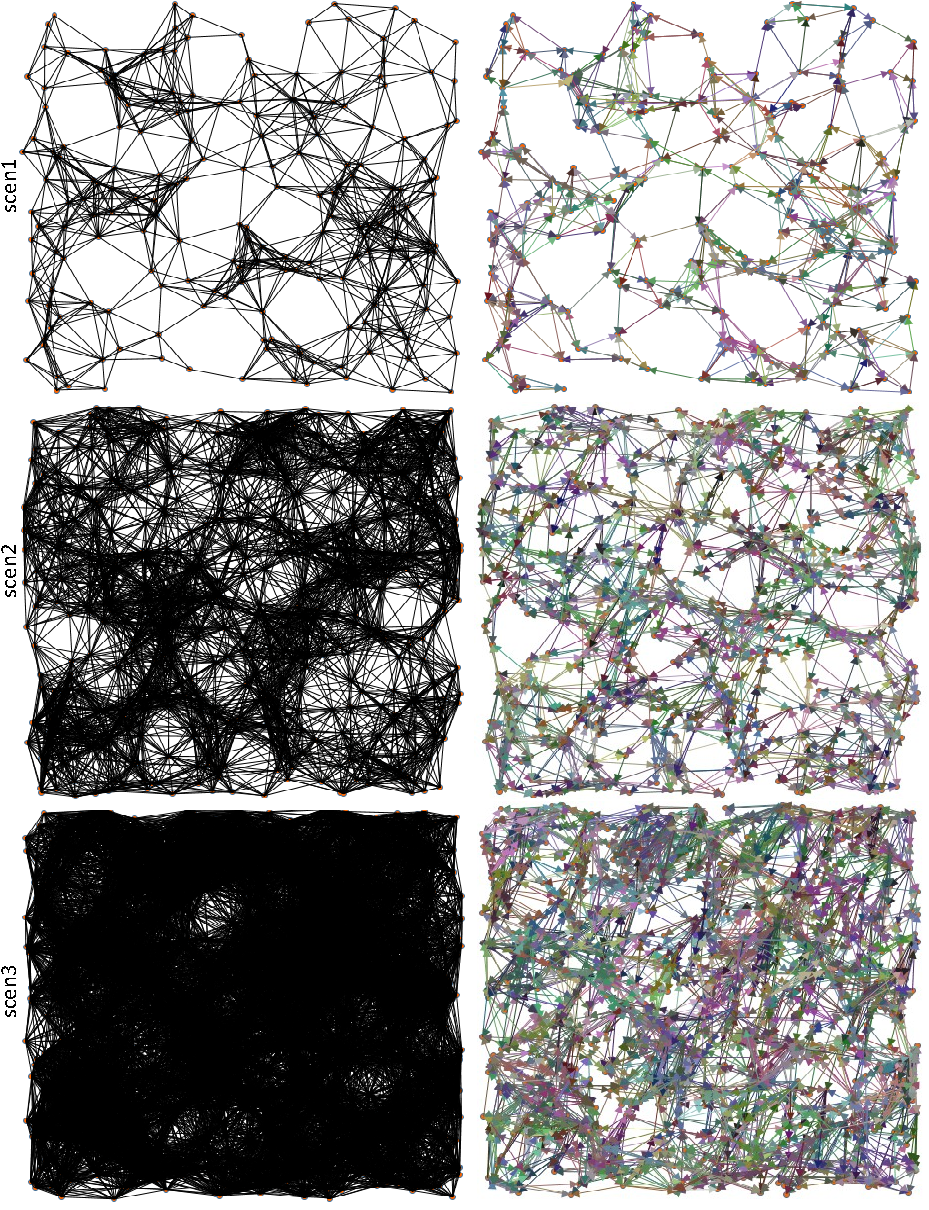
\includegraphics[width=\columnwidth]{nanonet.pdf}
\caption{Traffic regulation for 3 scenarios: 200 nodes, 500 nodes and 1000 nodes}
\label{nanonet}
\end{figure}

\begin{figure}[h]
\centering
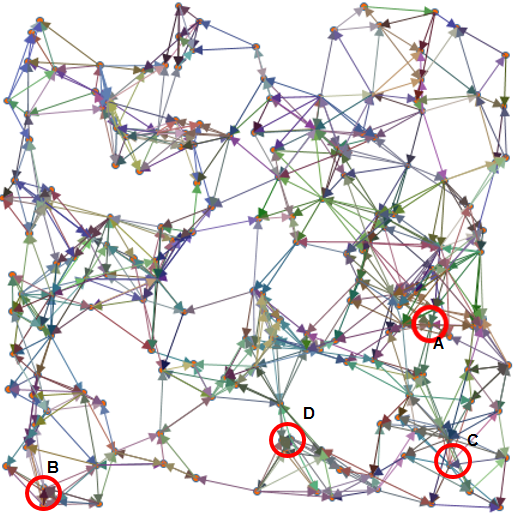
\includegraphics[width=\columnwidth]{broadcast.png}
\caption{4 cases of broadcast source nodes in scenarios 1 and 3}
\label{broadcast}
\end{figure}

\section{Conclusion and perspectives}
Dans cette article nous avons étudié l'opportunité d'optimiser la topologie logique d'une réseau nano ultra-dense. 
\begin{thebibliography}{1}

\bibitem{todo}
TO DO

\end{thebibliography}





% that's all folks
\end{document}